\chapter{Pairing-Based Contact Discovery}
\label{chap:system}

% TODO redo structure
\paragraph{} In this chapter we present the architecture for our contact discovery scheme (\autoref{sec:architecture}). We then provide outlines of security proofs (\autoref{sec:security}), theoretical performance evaluations (\autoref{sec:performance}) and show how our system maps onto real-world applications such as end-to-end encrypted messaging and mobile-first cryptocurrencies (\autoref{sec:applications}).


\section{Formal problem statement}
\label{sec:probstatement}

\paragraph{} First, we provide a formal definition for the problem of contact discovery. User $A$ is registered to a third-party application from which she receives an opaque account identifier $\acc_A$, an address $\addr_A$ and a secret/public key pair $(\sk_A,\pk_A)$. User $A$ also holds a human-readable discovery identifier $\id_A$ (mobile phone number or an email-address) and a list of contacts. We represent $A$'s address book as a set of discovery identifiers $\contacts{A}$. We assume that users exchanged discovery identifiers through out-of-bound communication but are unable to exchange cryptographic material, including their public keys and addresses. Thus for all users $B$ such that $\id_B \in \contacts{A}$ and $\id_A \in\ \contacts{B}$, $A$ wishes to learn the tuple $(\addr_B, \pk_B)$.

\section{Service architecture}
\label{sec:architecture}

\paragraph{} The foundational design principle for our contact discovery scheme is to provide users with the means to perform contact discovery locally. As we have seen in \autoref{chap:litreview}, sending a client the full list of registered users in a probabilistic data structures such as Bloom and Cuckoo filters requires the client to download and store large amounts of data. Instead, we follow an approach similar to the IBKE protocols and is closely related to the NI-IBKE described in \cite{LRPRF}. Our scheme runs in three phases which we will investigate individually:
\begin{enumerate}
	\item \textbf{Setup:} a one-time step for each user. During the setup phase, a user interacts with the contact discovery service to obtain her unique cryptographic material.
	\item \textbf{Key derivation:} using this cryptographic material, the user is able to compute shared secret keys with any of her contacts knowing only their discovery identifier.	\item \textbf{Discovery:} using their shared secret key, a pair of users can establish a secure meeting point on an untrusted online cache, thus allowing for asynchronous contact discovery.
\end{enumerate}

\noindent \autoref{fig:diagram} shows a diagram of the process described above.

\begin{figure}[H]
	\begin{center}	
	  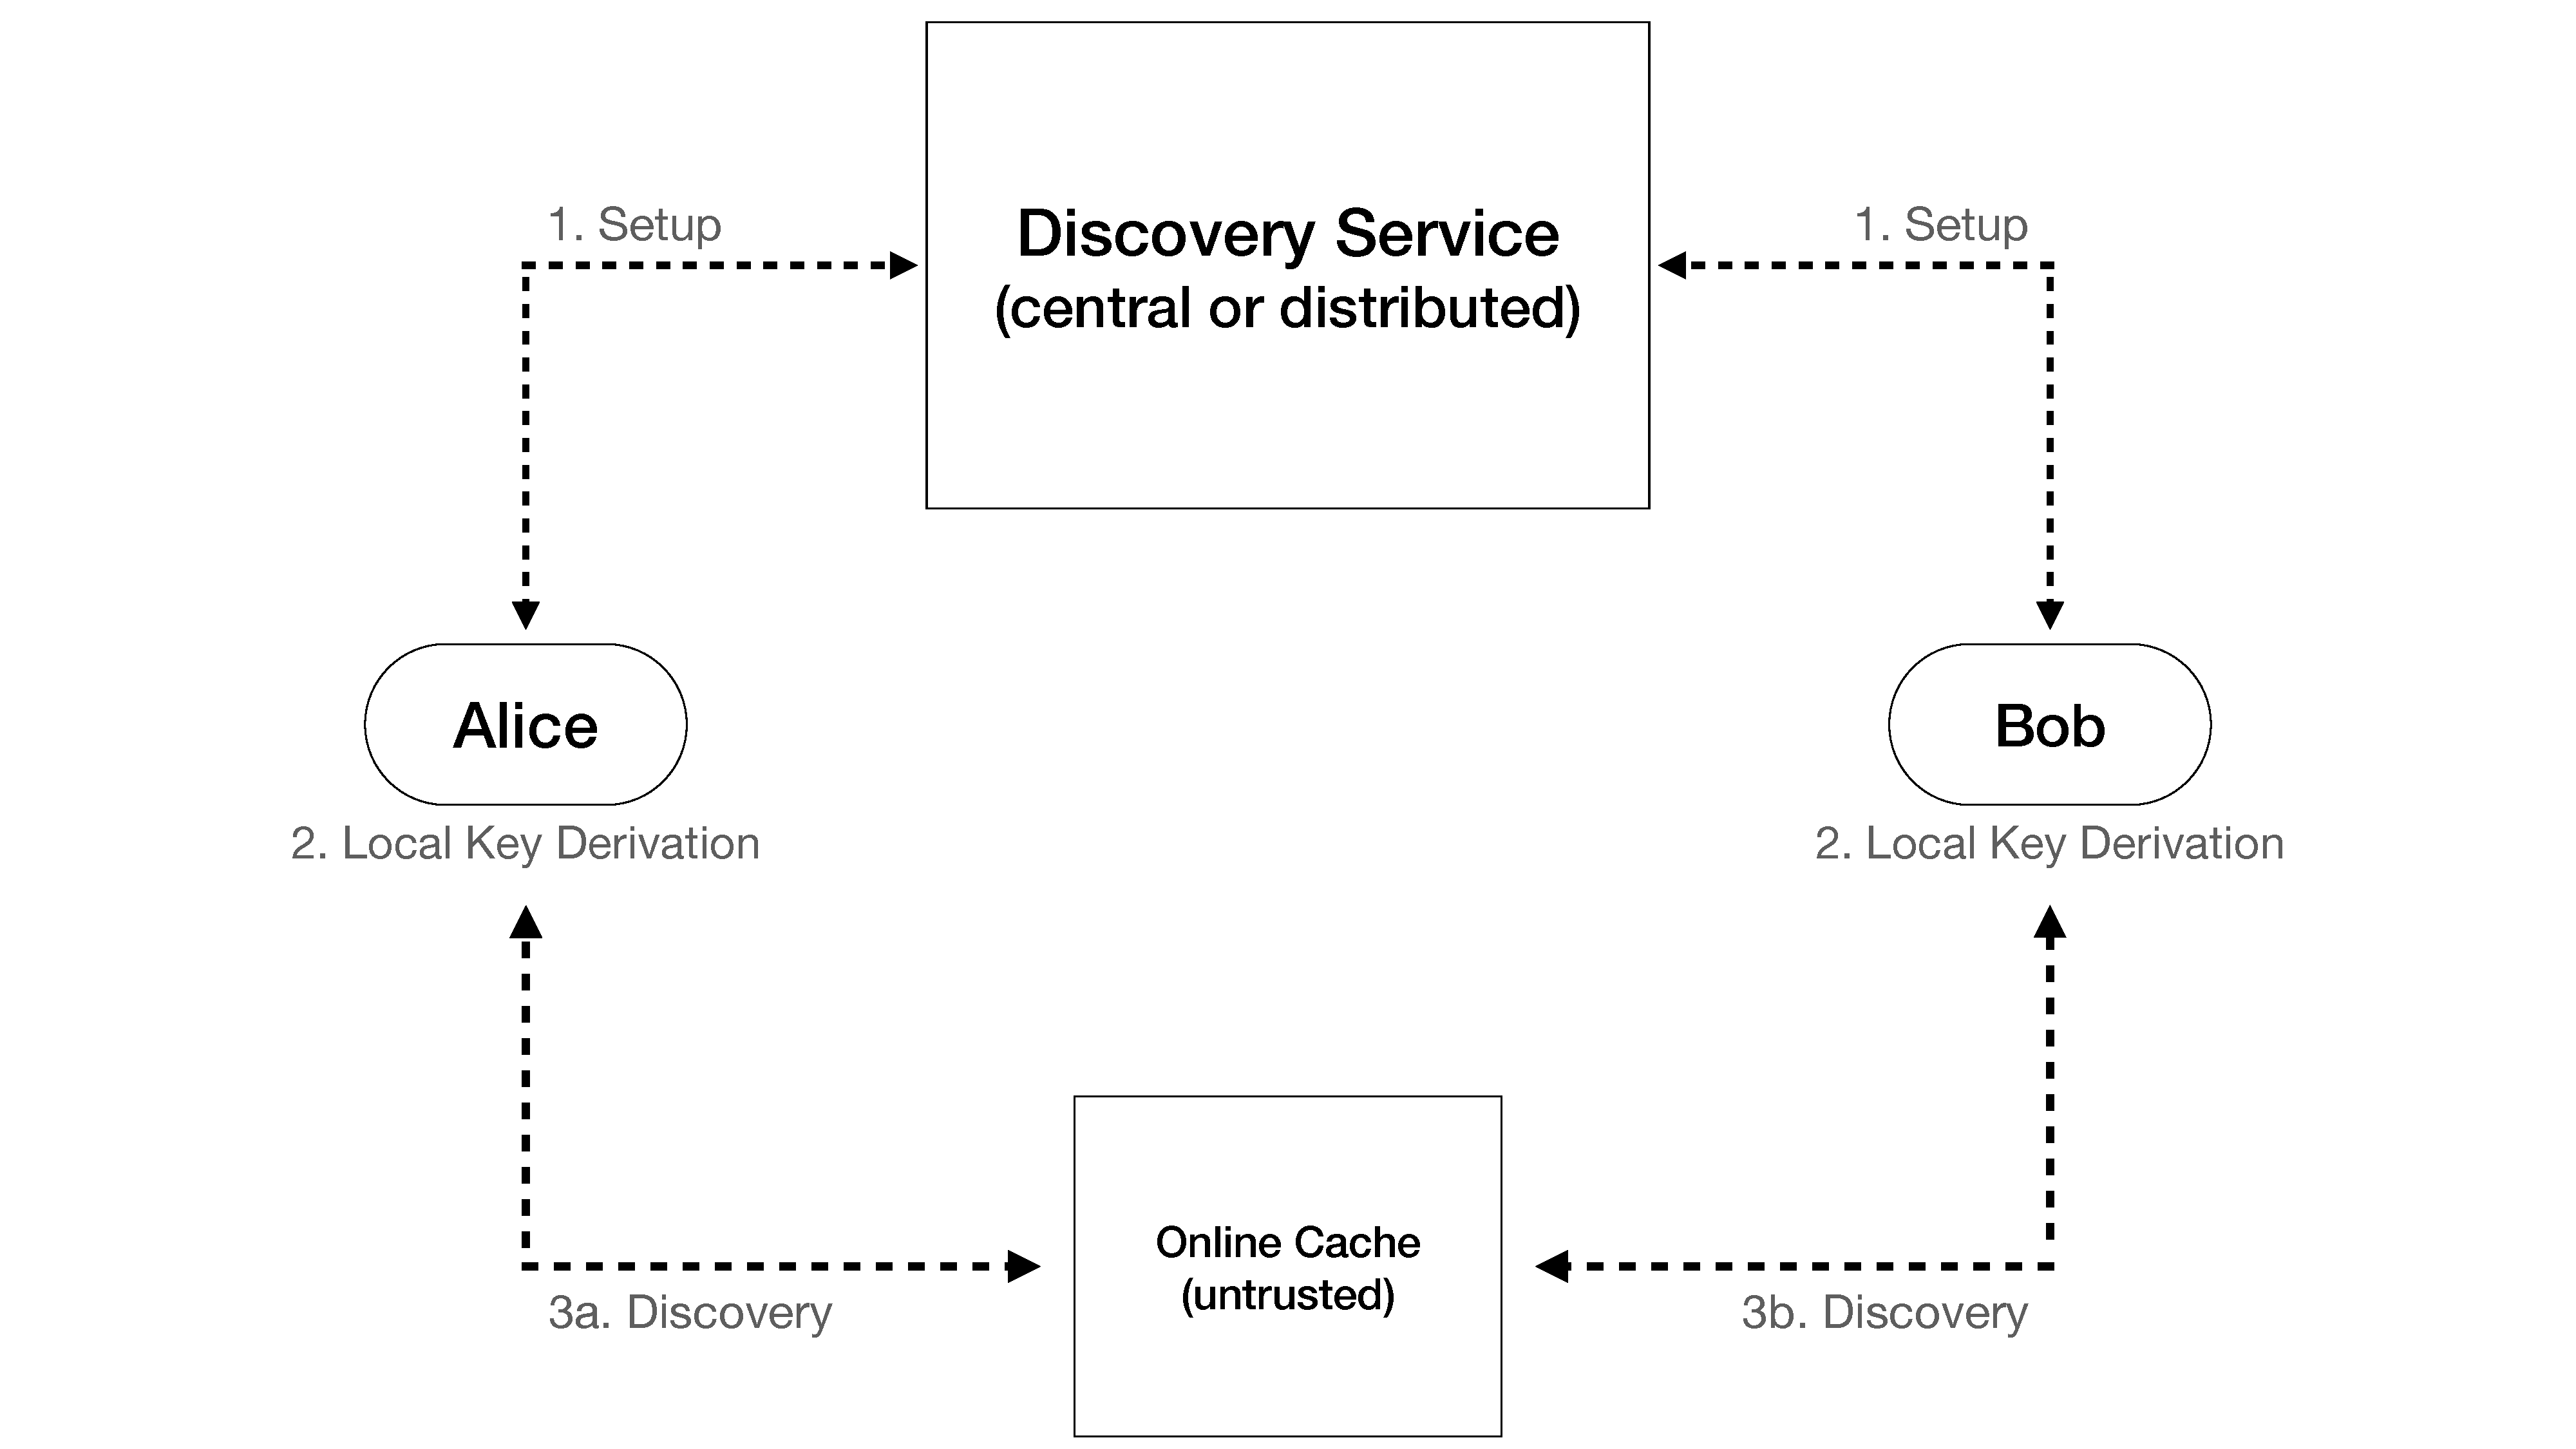
\includegraphics[width=\textwidth]{figures/system}
	  \caption{Contact discovery between a pair of users Alice and Bob, including setup. Numbers indicate the order of execution}
	  \label{fig:diagram}
	 \end{center}
 \end{figure}

	\subsection{Actors, assets and notation}
	
		\noindent We make a brief aside to clarify the actors and assets present in our scheme:		
		\begin{itemize}
			\item \textbf{Users:} each user $A$ holds an opaque account identifier $\acc_A$, an address $\addr_A$, a key pair $(\sk_A,\pk_A)$, a discovery identifier $\id_A$ and an address book $\contacts{A}$ (see \autoref{sec:probstatement}). We denote $\mathcal{ID}$ the set of all existing discovery identifiers.
			\item \textbf{Discovery Service:} the discovery service is a distributed entity. We denote the set of all servers as $\mathcal{S}$ and the $i$-th server as $S_i$. All $n$ servers have jointly executed a $(t,n)$-distributed key generation algorithm such as to hold shares $s_i$ of an unknown master secret key, which we denote $s$. Furthermore, each server holds a list of tuples $(\acc, \pk)$ for all registered users.
			\item \textbf{Online Cache:} the online cache may be operated by the discovery scheme or by a third party and is assumed to be untrusted. Its role is to manage key-value pairs. One possible implementation of such a cache is to follow the DNS-based approach of Papadopoulos \textit{et al.} \cite{Papadopoulos18}.
			
			\end{itemize}
			
		\noindent Next we define the cryptographic setting for our scheme. For a security parameter $\lambda$:
		\begin{itemize}
			\item $\Gzero, \Gone, \Gt$ are three cyclic groups of prime order $q > 2^{\lambda}$ such that there exists a pairing $e : \Gzero \times \Gone \rightarrow \Gt$.
			\item $H_0: \mathcal{ID}\rightarrow \Gzero$  and $H_1: \mathcal{ID} \rightarrow \Gone$ are two public hash functions modelled as random oracles.
			\item $F: \mathbb{Z}_q \times \mathcal{ID}^2  \rightarrow \Gt$ is a left/right constrained PRF defined as: \begin{equation}
				F(k, (\id_A, \id_B)) = F_k(\id_A, \id_B)= \Pair{H_0(\id_A)}{H_1(\id_B)}^k
			\end{equation}
			\item $\mathbf{KDF}$ is a public, deterministic key derivation function.
			\item $\BTBLS$ is a blind $(t,n)$-threshold BLS signature scheme (see definition \autoref{def:BTBLS}). We denote this scheme's algorithms as $\BTBLS . \Keygen$, $\BTBLS . \Sign$, \textit{etc...} 
			\item $\SIG$ is a strong existentially unforgeable signature scheme which makes use of the third-party provided user keys $(\sk_A,\pk_A)$ and is composed of algorithms $\SIG . \Sign$ and $\SIG . \Verif$.
			\item The master secret key is set to an integer $s \in \mathbb{Z}_q$ chosen uniformly at random. We define two corresponding master public keys ${g_0}^s$ and ${g_1}^s$, for which there exists $i$ public shares denoted as ${g_0}^{s_i}$ and ${g_1}^{s_i}$ respectively.
			\item Let $n$ the number of servers ($n=|\mathcal{S}|$)) and $t$ a fixed threshold such that $1 \leq t \leq n$, we assume that the master secret key is shared according to a secure $t$-out-of-$n$ secret sharing scheme and that no single entity holds the master secret key.
		\end{itemize}

	\subsection{Key derivation}
	
		\paragraph{} We first introduce the essential key derivation step. In doing so, we provide the reader with the necessary material to understand the security constraints under which the initial setup phase operates.
		
		\paragraph{} For all users $B$ such that $\id_B \in \mathcal{C}_A$, user $A$ can compute shared key material with $B$ by evaluating $F_s(\id_A, \id_B)$ and $F_s(\id_B, \id_A)$. From the definition of left/right constrained PRFs, $A$ can do so with the constraining keys $\keyleft{\id_A}$ and $\keyright{\id_A}$:
		\begin{align}
			f_{AB} = F_s(\id_A, \id_B) &= \Pair{\keyleft{\id_A}}{H_1(\id_B)} \\
			f_{BA} = F_s(\id_B, \id_A) &= \Pair{H_0(\id_B)}{\keyright{\id_A}}
		\end{align} 
	
	\noindent Similarly, $B$ can evaluate $F$ at the same points using the constraining keys $\keyleft{\id_B}$ and $\keyright{\id_B}$:		
		\begin{align}
			f_{AB} = F_s(\id_A, \id_B) &= \Pair{H_0(\id_A)}{\keyright{\id_B}} \\
			f_{BA} = F_s(\id_B, \id_A) &= \Pair{\keyleft{\id_B}}{H_1(\id_A)} 
		\end{align}
	
\noindent Using this key material, $A$ and $B$ can establish a symmetric secret key using a standardised key derivation function:
	\begin{equation}
		k_{AB} = k_{BA} = \mathbf{KDF}\left(f_{AB} \xor f_{BA}\right) = \mathbf{KDF}(f_{BA} \xor f_{AB})
	\end{equation}
	
	\paragraph{A note on security --} The constraining keys $\keyleft{\id_A}$ and $\keyright{\id_A}$ allow to compute every symmetric key that $A$ may establish with her contacts. As such, those \textbf{constraining keys must remain private} to $A$. The consequences of a leak range from impersonation to a total leak of $A$'s address book and are further detailed in \autoref{sec:security}.
	
	\subsection{Discovery}
	
		\paragraph{} Using their shared key material $(k_{AB}, f_{AB}, f_{BA})$, users $A$ and $B$ can determine secret memory locations on the online cache to leave an encrypted message for each other. Let $\enc$, $\dec$ be a secure symmetric encryption scheme and $H$ a hash function modelled as a random oracle, we define two cache operations $\mathbf{Write}$ and $\mathbf{Read}$:
		\begin{itemize}
			\item $\mathbf{Write}(f_{AB})$: store the key-value pair $(H(f_{AB}), \enc_{k_{AB}}(\pk_A || \addr_A))$ on the online cache.
			\item $\mathbf{Read}(f_{BA})$: retrieve the key-value pair $(H(f_{BA}), c_{BA})$. If $B$ has already run the discovery phase of our scheme then $c_{BA} = \enc_{k_{BA}}(\pk_B||\addr_B)$. Decrypt $c_{BA}$ using the key $k_{AB} = k_{BA}$.
		\end{itemize}
		
		\paragraph{} Using these two operations, $A$ is able to leave a message for $B$ to find ($\mathbf{Write}$) and check whether $B$ has previously completed the contact matching process ($\mathbf{Read}$ at the address $H(f_{BA})$). Both users regularly check the relevant memory locations for a message. Once both users have completed the contact discovery process, they will hold each other's public keys and address, allowing them to communicate securely.
	
	\subsection{Setup}
	\label{sec:setup}
		
		\paragraph{}  The setup stage serves to provide user $A$ with the constraining keys $k_{\id_A,\mathrm{LEFT}}$ and $k_{\id_A,\mathrm{RIGHT}}$. Consequently, the setup is a security-critical task. As we have shown in \autoref{eq:constrkeys}, under our construction of $F$ the constraining keys can be expressed as:
		\begin{equation}
			k_{\id_A,\mathrm{LEFT}} = H_0(\id_A)^s \quad \mathrm{and} \quad k_{\id_A,\mathrm{RIGHT}} = H_1(\id_A)^s
		\end{equation}
		
		\noindent These constraining keys are equivalent to BLS signatures on $\id_A$ by at least $t$ out of $n$ servers of the discovery service. Notice that the service needs to produce signatures under both variants of the BLS scheme: one with signatures in $\Gzero$ and one with signatures in $\Gone$.
		
		
		\paragraph{} The setup protocol between user $A$ and a server $S_i$ is described as follows:
		\begin{enumerate}
			\item $S_i$ issues a challenge $c$
			\item $A$ chooses a random blinding factor $\alpha \sample \mathbb{Z}_q$ and sends $\acc_A$, $\mathbf{sig}_A \leftarrow \SIG.\Sign(\sk_A, \acc_A || c)$, $\sigma_{\alpha,0} \leftarrow H_0(\id_A)^\alpha$, $\sigma_{\alpha,1} \leftarrow H_1(\id_A)^\alpha$ to $S_i$.
			\item Upon reception of $A$'s request, $S_i$ retrieves the associated public key and checks that the signature $\mathbf{sig_A}$ is valid:
			\begin{equation}
				\SIG.\Verif(\pk_A, \acc_A||c, \mathbf{sig}_A) = 1
			\end{equation}
		\item If the check succeeds, $S_i$ sends $\widehat\sigma_{i,0} \leftarrow {\sigma_{\alpha,0}}^{s_i}$ and $\widehat\sigma_{i,1} \leftarrow {\sigma_{\alpha,1}}^{s_i}$ to $A$.
		\item Using $S_i$'s public keys $({g_0}^{s_i}, {g_1}^{s_i})$, $A$ checks the following equalities:
		\begin{align}
			\label{eq:usercheck0}
			\Pair{\widehat\sigma_{i,0}}{g_0} &= \Pair{H_0(\id_A)^\alpha}{{g_0}^{s_i}} \\
			\label{eq:usercheck1}
			\Pair{g_1}{\widehat\sigma_{i,1}} &= \Pair{{g_1}^{s_i}}{H_1(\id_A)^\alpha}
		\end{align}
		\item If the checks succeed (in other words, if $A$ receives valid signatures from the service), $A$ removes the blinding factor $\alpha$ to obtain $H_0(\id_A)^{s_i}$ and $H_1(\id_A)^{s_i}$.
		\end{enumerate}
		
	
	\noindent $A$ repeats the above procedure with at least $t$ servers. Using the obtained signature shares, $A$ can recover the full signatures $H_0(\id_A)^s$ and $H_1(\id_A)^s$ using $\BTBLS.\Combine$.
	
	
	\paragraph{} This completes our description of the contact discovery scheme. We have seen how the setup process allows users to obtain their private constraining keys. Using those keys, users can locally and asynchronously derive shared key material with their contacts by evaluating a left/right constrained PRF at specific points. Finally, using the shared key material, users can leave and read messages from an untrusted online cache, thus completing the contact discovery process.


		
%\fbox{
%	\procedure{Setup}{%
%		\textbf{user } A  \< \<\textbf{server } S \\
%		\alpha \sample \mathbb{Z}_q \< \\
%		\mathbf{sig}_A = \Sign(\sk_A, \acc_A) \< \\
%		\<\sendmessageright{top={$\acc_A,\mathbf{sig}_A, H_0(\id_A)^\alpha, H_1(\id_A)^\alpha$} } \\
%		\<\< \text{If } \Verif(\pk_A, \acc_A, \mathbf{sig}_A) = 0 \\
%		\<\< \qquad\textbf{Abort}\\
%		\<\< \text{Else}\\
%		\< \sendmessageleft{top={$(H_0(\id_A)^\alpha)^s, (H_1(\id_A)^\alpha)^s$}} 
% }
% }


\section{Privacy}
\label{sec:security}


\paragraph{} We will now evaluate the privacy guarantees of our scheme when there are strictly less than $t$ malicious servers. Our scheme hides the links between users as long as the decisional bilinear Diffie-Hellman assumption holds for the pairing $e$, the master secret key $s$ does not leak and both constraining keys $\keyleft{X}, \keyright{X}$ are known only to user $X$. We present the threat model, potential attacks, outlines of security proofs as well as the consequences of a security breach.



	\subsection{Threat model}
	\paragraph{} An adversary $\Tadv$ wishing to break our scheme's privacy property aims to gain information about the contents of any user's address book. This goal is equivalent to determining whether $\id_B \in \contacts{A}$, for any user $A$ and any identifier $\id_B$ that is not owned by $\Tadv$. $\Tadv$ is characterised as:
	\begin{itemize}
		\item having access to all public information.
		\item having access to the present and past states of the online cache.
		\item may eavesdrop on any communication between the users, servers and online cache.
		\item may spawn any number of users for which $\Tadv$ owns the discovery identifier.
		\item may control up to $t-1$ servers in the discovery service.
	\end{itemize}
	
	\noindent Notice that we are working under the assumption that discovery identifiers are correctly linked to the users who own them. We discuss ways in which this assumption can be upheld in practice in \autoref{sec:impersonation}, under ``\textbf{Impersonating a user}''
	
	\subsection{Proof outline}
	
	\paragraph{} To guide our analysis, we provide an attack tree\footnote{as defined by Schneier \cite{attacktree}} against the privacy property of our scheme in \autoref{fig:attacktree}. The root node represents the attacker's goal and each child node represents an option to solve the problem indicated in the parent node. Consequently, leaf nodes represent the attacker's entry points: breaking the security of $F$, obtaining the master secret key $s$, forging BLS signatures on another user's discovery identifier, impersonating a user or computing the shared key material $(k_{AB}, f_{AB}, f_{BA})$. We will therefore consider each leaf node and show that our scheme is resistant against these attacks.
	
	
		\begin{figure}[H]
			\begin{center}
				\begin{center}
	

\begin{forest}
for tree={
  draw,
  minimum height=1cm,
  anchor=north,
  align=center,
  child anchor=north
},
[{Learn whether $\id_B \in \contacts{A}$}, align=center, name=SS
  [{Distinguish key-value pair\\ $(H(f_{AB}), \enc_{k_{AB}}(\pk_A || \addr_A))$\\ on online cache from random}, name=PDC
    [{Distinguish $f_{AB}$ from random}
    	[Break security\\ property of $F$\\ (definition \autoref{def:lrPRFsec})]
    	[Obtain $s$]
    	[{Obtain $A$'s\\ constraining keys}
    		[Forge BLS signatures]
    		[Impersonate $A$]
    	]
    ]
    [Decrypt $\enc_{k_{AB}}(\pk_A || \addr_A))$
    	[Compute $k_{AB}$]
    ]
  ]
]
\end{forest}

\end{center}
				\caption{Attack tree against our discovery scheme. Branches represent ``OR'' statements}
				\label{fig:attacktree}
			\end{center}
		\end{figure}

	
	
%		\paragraph{} Our scheme reduces the contact discovery problem to the evaluation of a left/right constrained PRF at two specific points, namely $(\id_A, \id_B)$ and $(\id_B, \id_A)$. Indeed an adversary trying to uncover a link between users $A$ and $B$ without computing their shared key material will face two obvious hurdles. Firstly, such an adversary will be unable to find $A$ and $B$'s meeting point on the online cache other than by exhaustively iterating through all possible location. Furthermore, since $H$ is modelled as a random oracle, this adversary will be unable to distinguish this location from any other. The second issue is that the value stored in that location is encrypted under $k_{AB}$. Therefore, to uncover the link between $A$ and $B$, an adversary will need to evaluate the left/right constrained PRF at the correct points.
		
		
%		\paragraph{} We provide a formal definition of secure left/right constrained PRFs by using an attack game. We will then show that the construction used in our scheme meets the security definition.
		
		\subsubsection{Security of our PRF construction}
		
		\paragraph{} We will first show that our construction for the left/right constrained PRF using an asymmetric pairing is secure as per definition \autoref{def:lrPRFsec}. Our construction is closely related to the one presented by Boneh and Waters \cite{LRPRF}. As such our proof sketch makes use of very similar ideas.
		
		\begin{theorem}
			The PRF $F$ defined as $F(k, (x,y)) = \Pair{H_0(x)}{H_1(y)}^k$ is a secure constrained PRF with respect to its constraining keys assuming the decisional bilinear Diffie-Hellman assumption holds for $e$ and the functions $H_0$ and $H_1$ are modelled as random oracles.
		\end{theorem}
		
		\begin{proof}[\textbf{Proof sketch}]
			We assume for contradiction the existence of a probabilistic polynomial-time adversary $\adv$ that distinguishes $F$ from random as in definition \autoref{def:lrPRFsec}, however $\adv$ is limited to a single $\mathsf{Challenge}$ query. We can then construct an adversary $\bdv$ that breaks the decisional bilinear Diffie-Hellman (DBDH) assumption.\\
			
			Given $(g_0, g_1, u_0 \leftarrow {g_0}^\alpha, u_1 \leftarrow {g_1}^\alpha, v_0 \leftarrow {g_0}^\beta, w_1 \leftarrow {g_1}^\gamma, z^{(b)})$, $\bdv$'s goal is to determine whether $z^{(b)} = z^{(0)} = {g_0}^{\alpha\beta\gamma}$ or $z
			^{(b)} = z^{(1)} = {g_0}^\delta$, where $\delta \sample \mathbb{Z}_q$ (see Attack Game \autoref{att:DBDH} in \autoref{ap:coCDH}). Using the pairing operation, this game can be viewed as distinguishing the output of $F$ from a random element of $\Gt$. Indeed let $b,c \in \mathcal{X}$ such that $H_0(b) = {g_0}^\beta$ and $H_1(c) = {g_1}^\gamma$, then:
			\begin{equation}
				\Pair{\Smallz{b}}{g_1} =
				\begin{cases} \Pair{g_0}{g_1}^{\alpha\beta\gamma} = \Pair{{g_0}^\beta}{{g_1}^\gamma}^\alpha =  F(\alpha, (b, c)), & \text{if } b=0 \\
				 \Pair{g_0}{g_1}^\delta	= {g_T}^\delta, & \text{if } b=1
				\end{cases}
			\end{equation}
			Thus, $\bdv$ will run $\adv$ as a sub-routine and must therefore emulate its oracles, namely $F.\mathsf{eval}$, $F.\mathsf{constrain}$, $\mathsf{Challenge}$ and oracles for the hash functions $H_0,H_1$. \\
			
			When $\adv$ issues a query to $H_0(x)$, $\bdv$ chooses a consistent random $\widehat x \sample \mathbb{Z}_q$ and sets $H_0(x) \leftarrow {g_0}^{\widehat x}$. To one of $\adv$'s queries to $H_0$ which we denote $x^*$, $\bdv$ responds with $H_0(x^*) \leftarrow v_0$. Queries to $H_1$ are answered in a similar fashion where one query is responded to with $H_1(y^*) \leftarrow w_1$. Using these values, queries to $F.\mathsf{constrain}(x,LEFT)$ where $x\neq x^*$ are answered with $k_{x,LEFT} \leftarrow  {u_0}^{\widehat x}$. Notice that as required
				$$ {u_0}^{\widehat x} = ({g_0}^\alpha)^{\widehat x} = {g_0}^{\alpha \widehat x} = ({g_0}^{\widehat x})^{\alpha} = H_0(x)^\alpha$$
			Similarly, queries to $F.\mathsf{constrain}(y,RIGHT)$ where $y\neq y^*$ are answered with $k_{y,RIGHT} \leftarrow  {u_1}^{\widehat y}$. Queries to $F.\mathsf{eval}(x,y)$ are answered for $x \neq x^*$ or $y \neq y^*$ by building the constraining keys as it is done for the $F.\mathsf{constrain}$ oracle. Notice that $\bdv$ does not hold the values $\beta,\gamma$ and is therefore unable to answer queries to the $F.\mathsf{constrain}$ oracle for $(x^*, LEFT)$ and $(y^*, RIGHT)$, nor can it answer the $F.\mathsf{eval}$ query for $(x^*,y^*)$. This is in fact equivalent to starting Attack Game \autoref{att:lrPRF} with the set $C$ initialised to $\{(x^*,y^*)\}$. \\
			
			After $n$ queries to the $H_0$ oracle and $m$ queries to the $H_1$ oracle, $\adv$ will hold at most $n \times m$ pairs on which it could challenge.	 Some of these pairs may have been added to the set $V$ due to queries to $F.\mathsf{constrain}$ and $F.\mathsf{eval}$, and thus become ineligible for challenging. However, since the experiment started with $C = \{(x^*,y^*)\}$, we can be sure that $(x^*,y^*)$ is an eligible pair (remember that the attack game maintains the invariant $C \cap V = \emptyset$). Therefore, $\adv$ will challenge the pair $(x^*,y^*)$ with probability $p \geq \frac{1}{n\times m}$, to which $\bdv$ answers with $\Smallz{b}$. 
			
			If $b=0$, then $\Smallz{b} = F(\gamma, (x^*, y^*))$ and $\adv$ will answer as in experiment EXP(0). On the other hand if $b=1$, then $\Smallz{b} = {g_T}^{\delta}$ and $\adv$ will answer as in experiment EXP(1). Let $b'_\adv$ be the output of $\adv$, we define as $b'_\bdv \leftarrow b'_\adv$ the return value of $\bdv$. Thus
			\begin{equation}
				\Pr[b'_\bdv = b] \geq \frac{1}{n \times m} \times \Pr[b'_\adv = b]
			\end{equation}
			
			Given that $\adv$ is a probabilistic polynomial-time adversary, $n \times m$ must necessarily be polynomial in $\lambda$. Therefore, if $\adv$'s advantage is non-negligible then so is $\bdv$'s, thus breaking the DBDH assumption and yielding a contradiction.
		\end{proof}
		
\subsubsection{Computing $A$ and $B$'s shared key material}

\paragraph{} To compute $A$ and $B$'s shared key material, an attacker needs to compute $f_{AB}$ and $f_{BA}$. This is in fact a harder problem than the decisional problem investigated above. We have already shown that no probabilistic polynomial-time adversary can break the security of $F$ under the DBDH assumption. Similarly, no probabilistic polynomial-time adversary will be able to compute either $f_{AB}$ or $f_{BA}$ under the DBDH assumption without access to the relevant constraining keys or the master secret key.

\subsubsection{Obtaining the master secret key}

\paragraph{} Next, we consider the option for an attacker to obtain the master secret key $s$. It is part of our assumption that there are strictly less than $t$ malicious servers. Therefore, they do not meet the threshold required to construct the master secret key. An attacker aiming to break our scheme through this attack will need to steal at least one of the key shares.

\subsubsection{Forging a BLS signature}

\paragraph{} As we have seen in \autoref{sec:setup}, the service generates constraining keys by signing a user's discovery identifier. The signing algorithm is a blind $(t,n)$-threshold BLS algorithm. As per \autoref{th:blsforge}, the BLS signature is existentially unforgeable against chosen message attacks under the co-Computational Diffie Hellman assumption. This assumption is in fact a weaker than the DBDH assumption which is required for the left/right constrained PRF security.


\subsubsection{Impersonating a user}
\label{sec:impersonation}

\paragraph{} Impersonation attacks are the most threatening to our scheme and lead to open questions. We first describe the issue and offer two solutions, neither of which are fully satisfying. The attack is performed by running the setup process maliciously from the user side: upon receiving a challenge $c$, $\Tadv$ can send the tuple $(\acc_{\Tadv}$, $\SIG.\Sign(\sk_{\Tadv}, \acc_{\Tadv}||c)$, $H_0(\id_A)^\alpha$, $H_1(\id_A)^\alpha$). The server $S_i$ receiving this tuple will find that the signature $\SIG.\Sign(\sk_{\Tadv}, \acc_{\Tadv}||c)$ does verify for the specified account and challenge. Furthermore, $S_i$ will be unable to distinguish the blinded values $H_0(\id_A)^\alpha, H_1(\id_A)^\alpha$ from random elements in $\Gzero$ and $\Gone$ respectively. As such $S_i$ will issue partial constraining keys for $\id_A$ to $\Tadv$. Repeating this process with $t$ servers, $\Tadv$ will obtain the full constraining keys for user $A$.

\paragraph{} The first solution is for $A$ to transmit her discovery identifier in clear to $S_i$. The server can then use out-of-bound communication to verify that $A$ indeed owns $\id_A$ (possible techniques include sending a one-time code via text message or email). If $A$ proves that she owns $\id_A$, $S_i$ provides the partial signatures for that discovery identifier. Notice that under this approach, $A$ cannot blind the hash of her discovery identifier. Consequently, the communication between $A$ and $S_i$ must be encrypted to prevent an eavesdropping adversary from learning the signature share on $\id_A$. Furthermore, this identification method allows the servers to build a list of identifiers for the users registered to the mobile application. In some cases, this may be a breach of privacy.

\paragraph{} The second solution makes use of identification tokens to delegate the task of linking a user to their discovery identifier. Suppose an entity $V$ (centralised or distributed) is trusted to verify whether a user owns a discovery identifier. Using a secret key $v \sample \mathbb{Z}_q$ and the corresponding public keys ${g_0}^v$ and ${g_1}^v $, $V$ could issue ownership tokens in the form of BLS signatures $t_{0,A}= H_0(\id_A)^v, t_{1,A}=H_1(\id_A)^v$. These tokens can then be blinded and verified against a blinded discovery identifier $H_0(\id_A)^\alpha, H_1(\id_A)^\alpha$:
\begin{align}
	\label{eq:token0}
	\Pair{{t_{0,A}}^\alpha}{g_1} = \Pair{H_0(\id_A)^\alpha}{{g_1}^v} &\iff t_{0,A} = H_0(\id_A)^v \\
	\label{eq:token1}
	\Pair{g_0}{{t_{1,A}}^\alpha} = \Pair{{g_0}^v}{H_1(\id_A)^\alpha} &\iff t_{1,A} = H_1(\id_A)^v
\end{align}

\noindent Users can therefore send ${t_{0,A}}^\alpha$, ${t_{1,A}}^\alpha$ along with the setup tuple $(\acc_A$, $\mathbf{sig}_A$, $H_0(\id_A)^\alpha$, $H_1(\id_A)^\alpha)$, to allow each server to perform the checks in \autoref{eq:token0} and \autoref{eq:token1}. 

\paragraph{} While this method allows identification without revealing the discovery identifier to the contact discovery servers, it relies on a trusted verification entity $V$. In fact, this entity faces the same problem we were trying to avoid: it must output a BLS signature on an identifier only if the request was made by the identifier's owner. This raises the question of trust within our system. The contact discovery scheme can be made secure and oblivious to which user owns which discovery identifier. However, for that to happen, we need another entity to perform that check and gather private information about the users.

	\subsection{Consequences of a breach}
	
	\paragraph{} To conclude our investigation of the scheme's privacy properties, we evaluate the consequences of various breaches of the protocol. Let us first consider the scenario in which a pair of constraining keys $\keyleft{\id_A}, \keyright{\id_A}$ is leaked. Using these keys, an attacker will be able to compute the shared key material $(k_{AX}, f_{AX}, f_{BX})$ between $A$ and any other user $X$. The attacker is then able to:
	\begin{enumerate}[label=(\alph*)]
		\item check whether $X$ has written to the cache in location $H(f_{XA})$, thus uncovering whether $\id_A \in \contacts{X}$. Iterating over all $\id_X \in \mathcal{ID}$ allows to determine which users hold $\id_A$ in their contacts. 
		\item decrypt the message (if any) left by $X$ at location $H(f_{XA})$ using the key $k_{AX}$, thus linking $\id_X$ to an address and public key.
		\item check whether $A$ has written to the cache in location $H(f_{AX})$, thus uncovering whether $\id_X \in \contacts{A}$. Iterating over all $\id_X \in \mathcal{ID}$ allows to recover all of $A$'s contacts.
		\item overwrite the value that $A$ wrote in location $H(f_{AX})$ using the key $k_{AX}$. This allows the attacker to send any address and public key to $X$, thus hijacking any channel that $A$ and $X$ were wishing to establish.
	\end{enumerate}
	
	\paragraph{} Should only one of the constraining keys leak, the attacker will only be able to perform a subset of the actions above. Indeed, obtaining a $LEFT$ key only allows to compute $f_{AX}$. The attacker will therefore only be able to perform action (c). Similarly, obtaining only a $RIGHT$ key limits the attacker's possibilities to (a). In either case, these breaches represent a complete loss of privacy. Finally, obtaining the master secret key allows to compute any constraining key, thus allowing to perform the above operations for any pair of users.


\section{Theoretical performance evaluation}
\label{sec:performance}



	\paragraph{} In this section we present a brief evaluation of the scheme's efficiency. Importantly, we show that all computational costs grow linearly with respect to the input size. We estimate the computation time associated with each phase of our discovery scheme using benchmark timings from the elliptic curve pairing library MCL \cite{MCLLib} (see calculations in \autoref{app:perf}). These benchmark tests were performed on an iPhone 7 running iOS 11.2.1 (\autoref{table:benchmarks}) and an Intel Core i7 processor (3.6GHz) running Linux (\autoref{table:benchmarks_server}), executing operations over three Barreto-Naehrig (BN) elliptic curves with varying security parameters \cite{MCLBench}.  Notice that we are now working with elliptic curves and therefore adopt an additive notation for the group operation.
	
	
	

\begin{table}[H]
	\begin{center}
	\resizebox{0.68\textwidth}{!}{
		\begin{tabular}{l|c||c|c|c}
		Operation            		 & Notation 				     & BN254 & BN381\_1  & BN462  \\
		\hline
		Pairing           			 & $\mathbf{p}$ 				 &3.9   & 11.752 & 22.578 \\
		Addition in $\Gzero$ 		 & $\mathbf{add}_{\Gzero}$   &0.006 & 0.015  & 0.018  \\
		Point doubling in $\Gzero$   & $\mathbf{dbl}_{\Gzero}$   &0.005 & 0.01   & 0.019  \\
		Multiplication in $\Gzero$   & $\mathbf{mul}_{\Gzero}$   &0.843 & 2.615  & 5.339  \\
		Addition in $\Gone$ 		     & $\mathbf{add}_{\Gone}$    &0.015 & 0.03   & 0.048  \\
		Point doubling in $\Gone$    & $\mathbf{dbl}_{\Gone}$    &0.011 & 0.022  & 0.034  \\
		Multiplication in $\Gone$    & $\mathbf{mul}_{\Gone}$    &1.596 & 4.581  & 9.077  \\
		Hash to $\Gzero$             & $\mathbf{hash}_{\Gzero}$  &0.212 & 0.507  & 1.201  \\
		Hash to $\Gone$              & $\mathbf{hash}_{\Gone}$   &3.486 & 9.93   & 21.817 \\  
		\end{tabular}}
		\caption{Timing benchmarks for elliptic curve operations over three pairing-friendly curves (BN254, BN381\_1 and BN462) executed on an iPhone 7 running the MCL library \cite{MCLLib} on iOS 11.2.1. All timings are given in milliseconds. \cite{MCLBench}}
		\label{table:benchmarks}
	\end{center}
\end{table}
	
	{

\begin{table}[H]
	\begin{center}
	\resizebox{0.68\textwidth}{!}{
		\begin{tabular}{l|c||c|c|c}
		Operation            		 & Notation 				     & BN254 & BN381\_1  & BN462  \\
		\hline
		Pairing           			 & $\mathbf{P}$ 				 &2.446  & 7.353     & 14.596 \\
		Addition in $\Gzero$ 		 & $\mathbf{ADD}_{\Gzero}$   &0.007  & 0.01      & 0.014  \\
		Point doubling in $\Gzero$   & $\mathbf{DBL}_{\Gzero}$   &0.005  & 0.007     & 0.011  \\
		Multiplication in $\Gzero$   & $\mathbf{MUL}_{\Gzero}$   &0.479  & 1.529     & 3.346  \\
		Addition in $\Gone$ 		     & $\mathbf{ADD}_{\Gone}$    &0.013  & 0.022     & 0.033  \\
		Point doubling in $\Gone$    & $\mathbf{DBL}_{\Gone}$    &0.01   & 0.016     & 0.025  \\
		Multiplication in $\Gone$    & $\mathbf{MUL}_{\Gone}$    &0.989  & 2.955     & 5.921  \\
		Hash to $\Gzero$             & $\mathbf{HASH}_{\Gzero}$  &0.135  & 0.309     & 0.76   \\
		Hash to $\Gone$              & $\mathbf{HASH}_{\Gone}$   &2.14   & 6.44      & 14.249 \\ 
		\end{tabular}}
		\caption{Timing benchmarks for elliptic curve operations over three pairing-friendly curves (BN254, BN381\_1 and BN462) executed on an Intel Core i7 Processor clocked at 3.6GHz running the MCL library for Linux. All timings are given in milliseconds. \cite{MCLBench}}
		\label{table:benchmarks_server}
	\end{center}
\end{table}

}
	
	\subsubsection{Computational cost: Setup with identification tokens}
	
	\paragraph{} First, let us inspect the setup phase with identification tokens. This phase only needs to be performed once per user and per server. As such we will evaluate the computational cost of a single user-server interaction, then consider the scaling with respect to the total number of users $N$ and the threshold of servers $t$. We assume that users already hold a hash of their own discovery identifier. By inspection of the protocol, the setup phase requires: 
	\begin{quote}
		\textbf{User:} 2 multiplications in $\Gzero$, 2 multiplications in $\Gone$ (blind and unblind identifier), 4 pairing operations (\autoref{eq:usercheck0}, \autoref{eq:usercheck1}), one standard digital signature. Identification tokens introduce one additional multiplication in $\Gzero$, and one multiplication in $\Gone$ (blind tokens). After repeating these operations with enough servers to meet the system's threshold, a user is required to recombine $t$ partial BLS signatures in both $\Gzero$ and $\Gone$. Using Lagrange interpolation, each of these recombinations require $t$ multiplications and $t$ additions in their respective source group. We can now express the time spent by each user on computations for the setup phase as a function of $t$:
		\begin{equation}
			\mathrm{comp}_{\mathrm{setup, user}}(t) = t(4(\mathbf{mul}_{\Gzero} + \mathbf{mul}_{\Gone} + \mathbf{p}) + \mathbf{add}_{\Gzero} + \mathbf{add}_{\Gzero} + \mathbf{dsa}_S)
		\end{equation}
		\noindent where $\mathbf{dsa}_S$ is the time to execute the digital signature algorithm on a mobile device.
		
				
		\textbf{Server:} 1 multiplication in $\Gzero$, 1 multiplication in $\Gone$ (BLS signature in each source group) and one standard digital signature verification. Identification tokens introduce 4 additional pairing operations (\autoref{eq:token0}, \autoref{eq:token1}). We express the time spent by each server on computations for the setup phase as a function of $N$:
		\begin{equation}
			\mathrm{comp}_{\mathrm{setup, server}}(N) = N(4\mathbf{P} + \mathbf{MUL}_{\Gzero} + \mathbf{MUL}_{\Gone} + \mathbf{DSA}_V)
		\end{equation}
		\noindent where $\mathbf{DSA}_V$ is the time to verify the digital signature on a desktop computer.
	\end{quote}
	
	\paragraph{} Assuming we are using curve BN381\_1 and using realistic values for $\mathbf{dsa}_S$ and $\mathbf{DSA}_V$ (respectively $0.82$ ms and $3.02$ ms \cite{WolfSSl}) yields:
	\begin{alignat}{2}
		\mathrm{comp}_{\mathrm{setup, user}}(t) &= 76.66 \times t  \qquad &\mathrm{ms} \\
		\mathrm{comp}_{\mathrm{setup, server}}(N) &= 36.98\times N &\mathrm{ms}
	\end{alignat}
	
	\noindent For a threshold of servers set to $6$, a single user can complete the setup phase while spending less than 0.5 seconds performing local computations. Similarly, servers can setup a new user within tens of milliseconds. Launching our discovery service for an application with 10 million users can be done with slightly more 4 days of serial computations on a single Inter Core i7 processor. However, with no optimisations, an application with one billion users would require a roll out period of more than one year (approximately 1.2 years).
	
	\paragraph{} In order to render the service practical for widely used applications, we must investigate methods to optimise the server-side setup process. Firstly, processing computations in parallel on multiple, faster processors can reduce the roll out period by a large constant factor. Secondly, we can optimise the cryptographic checks. Indeed, the most costly operations performed by each server are the verifications of the identity tokens. These are in fact verification of BLS signatures, which can be aggregated to reduce the number of pairing operations needed \cite{BLSagg}. We can establish optimal batching strategies by placing assumptions on the rate of false signatures; however, such strategies are outside of the scope of this report. Promising approaches to establishing an optimal strategy may come from other fields of research \cite{covid}. 
	
	\subsubsection{Computational cost: Shared key derivation}
	
	\paragraph{} We now consider the local key derivation phase on a per-contact basis, before investigating how computations scale with the number of contacts $N_c$. A user must perform two evaluations of a left/right constrained PRF. Under our construction, this amounts to performing one hash to each source group and two pairing operations. Thus:
	\begin{equation}
		\mathrm{comp}_{\mathrm{key, user}}(N_c) = N_c(2\mathbf{p} + \mathbf{hash}_{\Gzero} + \mathbf{hash}_{\Gone})
	\end{equation}

	\paragraph{} Using the values from curve BN381\_1 in \autoref{table:benchmarks} yields  a very fast $34\mathrm{ms}$ per address book entry. Thus an initial computation over an address book of one thousand entries would only require 34 seconds of computations.
	
	\subsubsection{Concluding remarks}
	
	\paragraph{} The discovery phase makes use of standard cryptographic operations and is of lesser interest when estimating the computational costs of our scheme. However, a similar analysis of the scheme can be performed for communication costs. These are largely dependent on the type of mobile network that is being used as well as the availability of the servers and the online cache. We do not perform this analysis in our report, however we wish to emphasise that our scheme requires very few communications rounds to complete all three phases.
	
	
	\paragraph{} Overall, we have seen that all computations grow linearly with respect to their inputs. Using realistic numbers of registered users, we have seen that our service may be immediately applicable to relatively popular applications (in the range of tens of millions of users). For more popular applications such as WhatsApp, our system will require optimisations of the server-side setup process. Under our construction of the left/right constrained PRF, the most promising approach is to batch token verifications to reduce the number of pairing operations required. 
	
 	


\section{Applications}
\label{sec:applications}

\paragraph{} To conclude this chapter on our system's architecture, we provide a brief overview of its possible integrations into existing mobile applications. We first focus on Signal\footnote{\url{https://signal.org}}, an end-to-end encrypted messaging service. We then consider the integration with a decentralised payment system such as Celo\footnote{\url{https://celo.org}}.

\paragraph{} It is important to note that the same infrastructure can be used for multiple applications simultaneously. Indeed, each application can be represented by a different master secret key. Let $s_X$ and $s_Y$ be the master secret keys for applications $X$ and $Y$ respectively. Users $A$ and $B$ can interact with the discovery service under both keys to derive the shared secrets $F_{s_X}(\id_A, \id_B), F_{s_X}(\id_B, \id_A)$ to perform contact discovery for application $X$ and the shared secrets $F_{s_Y}(\id_A, \id_B), F_{s_Y}(\id_B, \id_A)$ to perform contact discovery for application $Y$. However, this once again raises the question of optimisation of the server-side setup process.

	\subsection{End-to-end encrypted messaging}
	
	\paragraph{} The Signal Protocol uses the ``X3DH'' (Extended Triple Diffie-Hellman) protocol to ``[establish] a shared secret between two parties that mutually authenticate each other'' \cite{Signal:X3DH}. Users $A$ and $B$ first exchange a set of public keys to then derive a shared secret. We can modify our discovery scheme such that the initial ciphertext left on the online cache contains the necessary public key information to perform the X3DH protocol. As the meeting point and encryption key are known only to $A$ and $B$, our scheme provides mutual authentication. Following this initial key establishment, the Signal Protocol can be followed as expected normally. This allows features such as the ``Double Ratchet'' algorithm to be used to provide secrecy to past and future messages in the event of a key leak \cite{Signal:Ratchet}. Such features allow to isolate the end-to-end encrypted channel from faults in the discovery scheme.
	
	\paragraph{} Signal also performs a phone number registration step which makes use of out-of-bound verification \cite{Signal:Reg}. This step is less documented, however its existence implies that Signal is able to issue identification tokens to its users, thus protecting our scheme from impersonation attacks. 
	
	\subsection{Mobile-first cryptocurrencies}
	
	\paragraph{} Celo is a decentralised payment system based on a blockchain architecture. Users can therefore send and receive transactions using account addresses - a 30+ character hexadecimal string. As Celo aims to bring fast payment systems to ``anyone with a smartphone'' \cite{Celo:Doc}, they provide a service which allows users to ignore these complex addresses and use phone numbers instead. This setting naturally maps to our contact discovery scheme (phone number as a discovery identifier linked to the Celo-provided secret key, public key and address).
	
	\paragraph{} Through its blockchain and the validators that run it during a given epoch, Celo offers a decentralised phone number attestation service \cite{Celo:Phone}. Once a user proves they own a phone number, a salted hash of the number and the associated Celo account are committed to the blockchain. Users can discover each other by issuing oblivious, rate-limited requests for a user's salt to then check the on-chain phone number attestation records.	
	
	\paragraph{} Instead, Celo could provide stronger privacy guarantees by issuing private identification tokens through its attestation system and delegating the contact discovery process. Our contact discovery service could then use the public keys associated to the combined secret key of the validators of a given epoch to verify these tokens. As this authentication step prevents impersonation attacks, our scheme can then run as described in this chapter. Doing so allows to securely link phone numbers to account addresses without committing this data to a public blockchain.
	
	
	
	
	
	
	
	
	
	
	
	
	
	
	
	
	
	
	
	
	
	
	
	
